\documentclass[a4paper, amsfonts, amssymb, amsmath, reprint, showkeys, nofootinbib, twoside]{revtex4-1}
\usepackage[english]{babel}
\usepackage[utf8]{inputenc}
\usepackage[colorinlistoftodos, color=green!40, prependcaption]{todonotes}
\usepackage[pdftex, pdftitle={Article}, pdfauthor={Author}]{hyperref}
\usepackage{amsthm}
\usepackage{mathtools}
\usepackage{physics}
\usepackage{xcolor}
\usepackage{caption}
\usepackage{hyperref}
%\hypersetup{colorlinks=true, linkcolor=blue, urlcolor = blue}
\usepackage{amsmath}
\usepackage{amssymb}
\usepackage{graphicx}
\graphicspath{Images}
\usepackage[left=23mm,right=13mm,top=35mm,columnsep=15pt]{geometry} 
\usepackage{adjustbox}
\usepackage{placeins}
\usepackage[T1]{fontenc}
\usepackage{float}
%\usepackage{longtable}
\usepackage{csquotes}
\usepackage{refstyle}
\usepackage{lipsum}

\begin{document}

\title{Study of Hydrogen spectra in Balmer series and determination of Rydberg's constant}
\author{Swaroop Ramakant Avarsekar}
\email{swaroop.avarsekar@niser.ac.in}
\affiliation{School of Physical Sciences, National Institute of Science Education and Research, HBNI, Jatni -752050, India}
\date{\today}

	
\begin{abstract}
This experiment aims to determine the wavelength of visible spectral lines in Balmer series of Hydrogen atom and thus determining Rydberg's constant. Mercury lamp is used to calibrate the spectrometer, then Hydrogen lines are observed. We obtained three spectral lines of Balmer series as $H_\alpha=(672.17\pm7.15) nm$, $H_\beta=(492.81\pm5.25) nm$, $H_\beta=(441.9\pm4.71) nm$ and determined Rydberg's constant as $(1.0947\pm0.0180) m^{-1}$.  $H_\alpha$ line corresponds to red line, $H_\beta$ line corresponds to green line,
$H_\gamma$ line corresponds to violet line of emission spectra of Hydrogen atom. 
\end{abstract}
	
\keywords{Emission, grating element, Rydberg's constant}
	
\maketitle

\section{Introduction and Theory}
Niels Bohr was one of the first person to theoretically deduce the empirical formula given by Rydberg for the wave number of spectral lines of Hydrogen atom. 

\begin{equation}
	\frac{1}{\lambda}=R\left[ \frac{1}{n_1^2}-\frac{1}{n_2^2}\right] 
\end{equation}
where $n_1=1, 2, 3...$ and $n_2=2, 3, 4...$ and R is Rydberg's constant=$1.097\times10^7 m^{-1}$

$$\text{Rydberg's constant}=\frac{e^4.m}{8\epsilon_o^2h^3c}$$

where $h$ is Planck's constant, $c$ is speed of light, $e$ is charge of electron

Using diffraction grating wavelength of the hydrogen spectral lines can be calculated with the help of spectrometer. Diffraction grating is the arrangement of the numerous parallel slits (N) with equal width (e) and spacing (b). The grating element is defined as g=(e+b) and N is the number of slits per unit length (N=1/g). The principal maxima is given by 
\begin{equation}
	g.sin \theta=m \lambda
\end{equation}

where $m$ is the order of principal maximum and $\theta$ is the angle of diffraction.



\section{Experiment}
\subsection{Apparatus}
Hydrogen and Mercury spectral tubes will be used as a light source. A grating or spectrometer is used to analyze the spectra. Torch may help while measuring angles. 
\subsection{Procedure}
Setup and collimate the spectrometer. Fix the grating element on the prism table. From mercury as lamp source, determine the grating element g, by observing the first order spectral lines on both sides of the spectrometer. Note down the readings by aligning the position of spectral lines. Determine the diffraction angle, $\theta$ for the spectrum and calculate g. Replace the Hg lamp with hydrogen source and repeat similar procedure for red green and violet first order spectral lines, to calculate the wavelength of each line and Rydberg constant. 

\begin{figure}[H] %  figure placement: here, top, bottom, or page
	\centering
	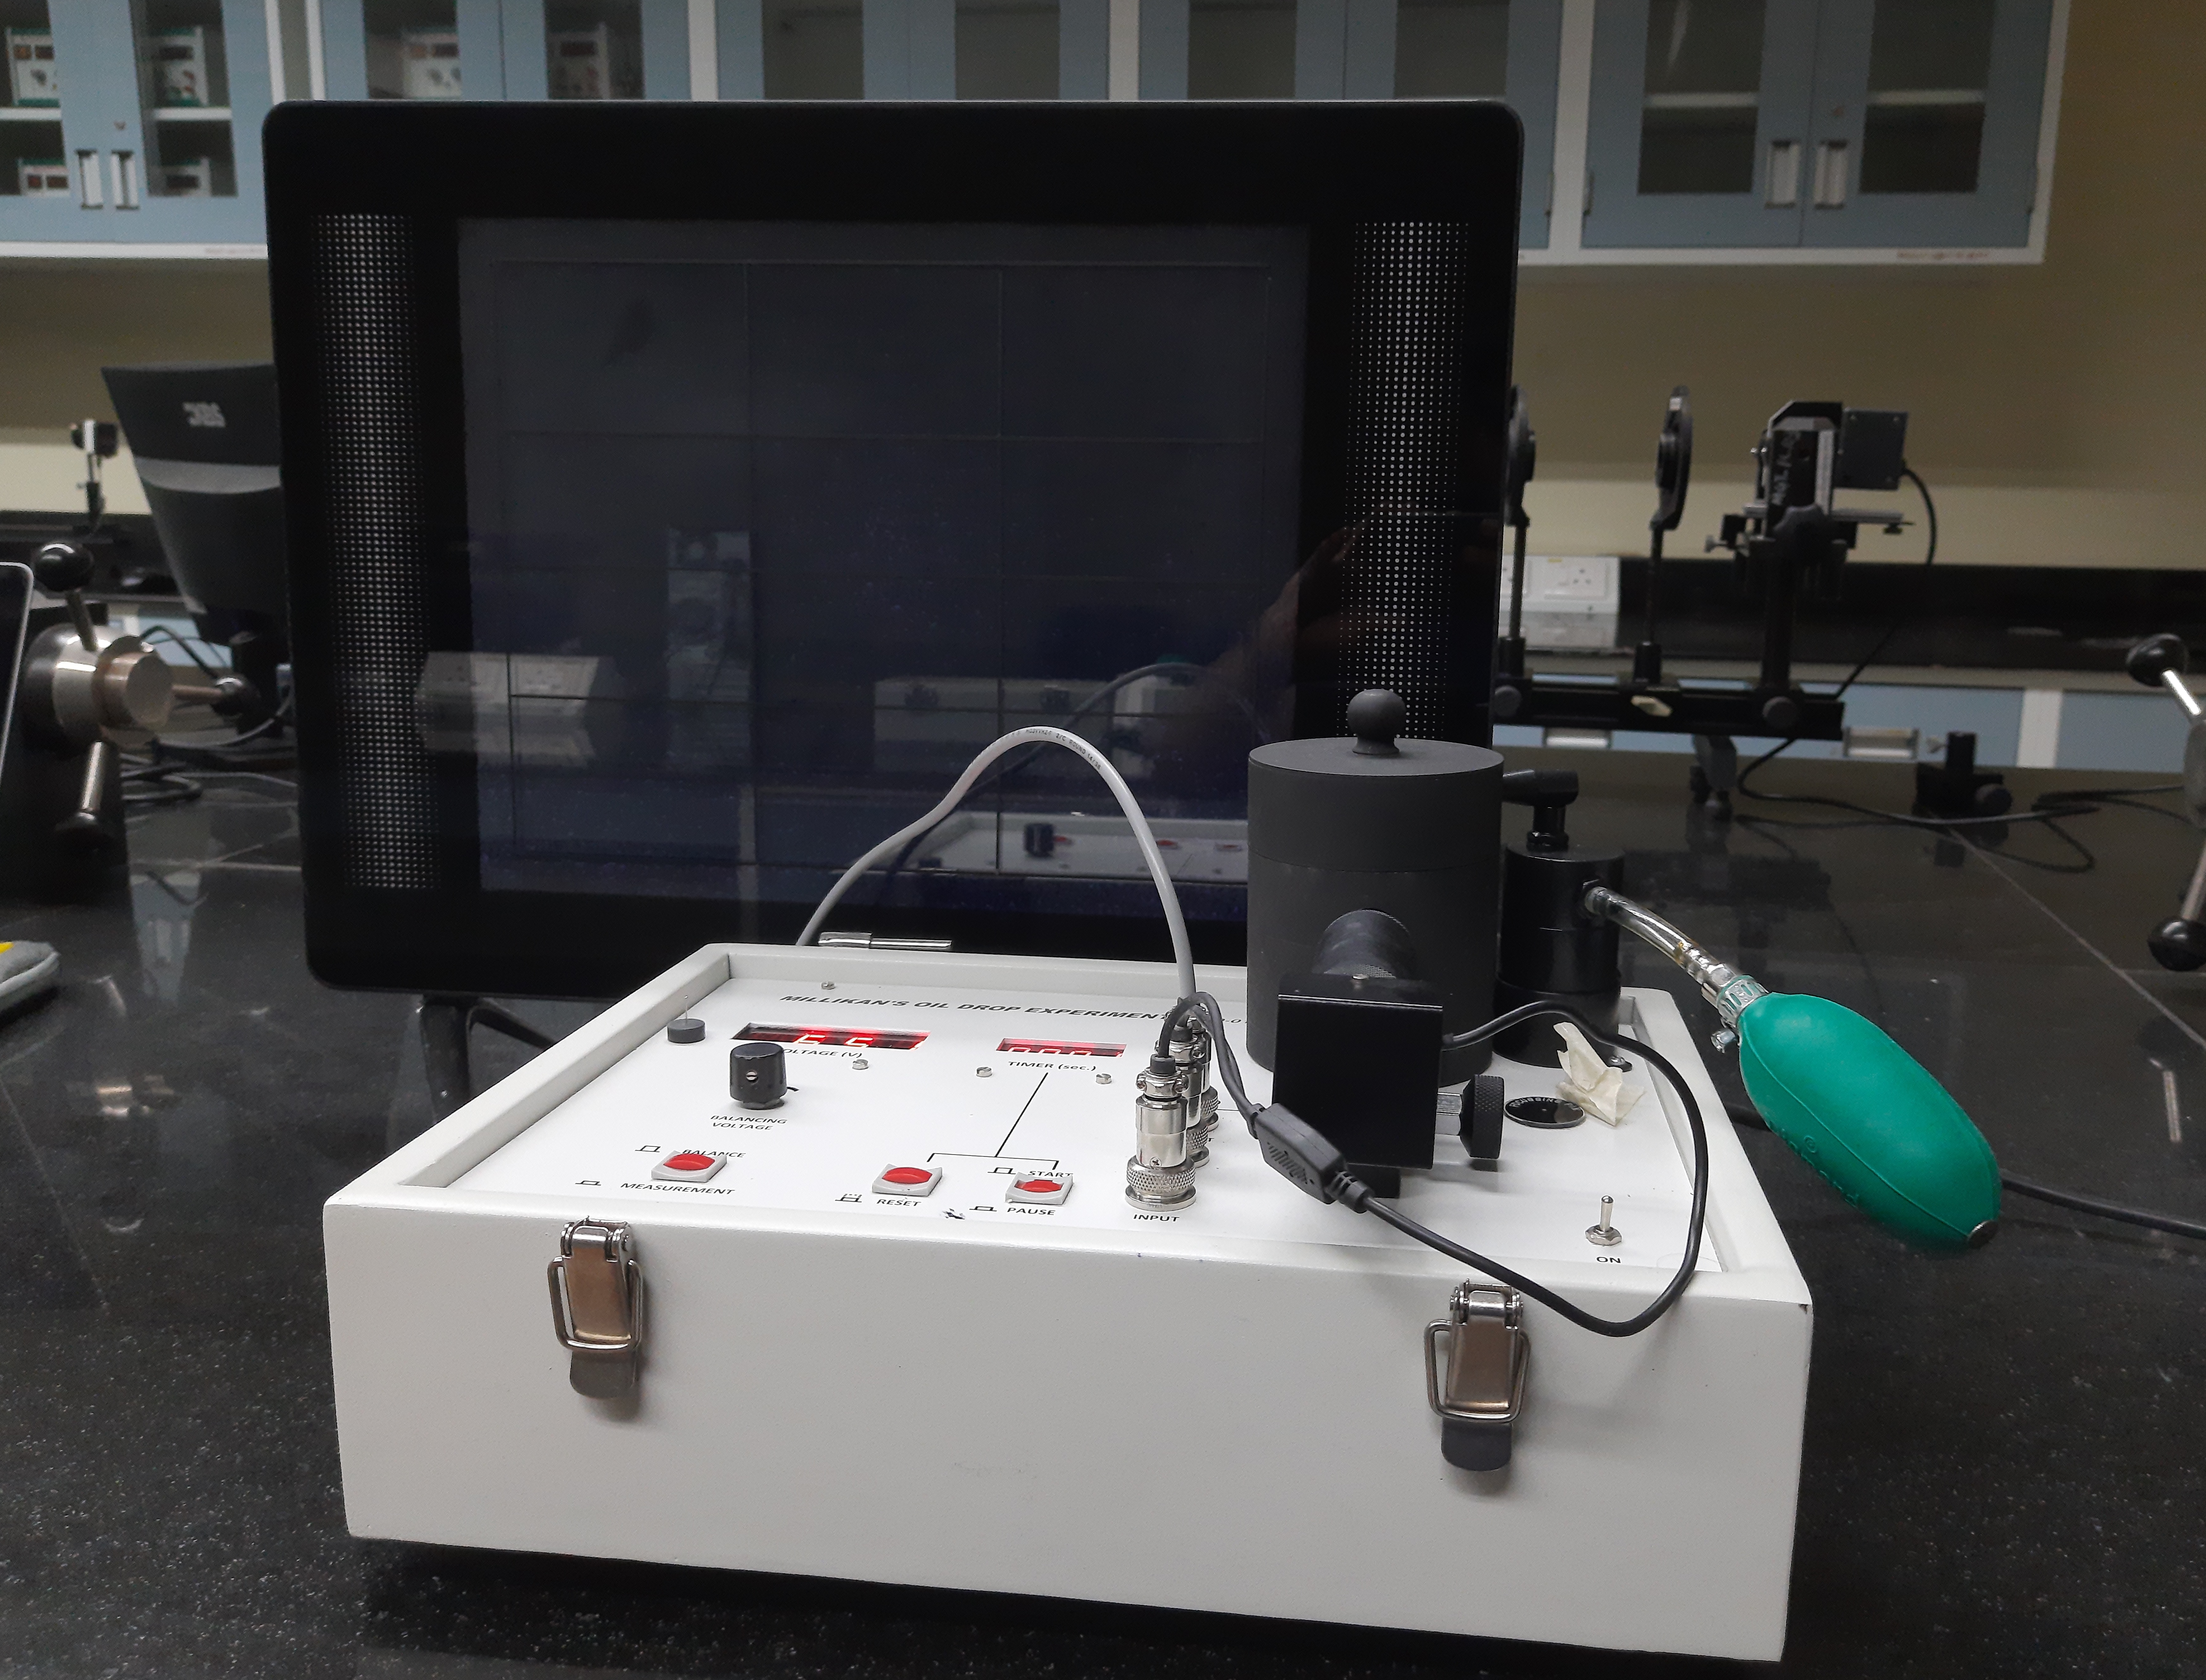
\includegraphics[width=8.5cm,height=7cm,angle=270]{1} 
	\caption{Schematic diagram for experimental setup}
	\label{1}
\end{figure}

\subsection{Precautions}
\begin{enumerate}
	\item {Do not touch the surface of diffraction grating.}
	\item {Always allow sufficient time for lamp to glow before taking readings}
	\item {Make sure you do not change the postion of spectrometer after set up}
	\item {Do not touch optical surfaces with fingers.}
	\item {Switch off the power supply before making any changes.}
\end{enumerate}


\section{Observation and Analysis}

\begin{figure}[H] %  figure placement: here, top, bottom, or page
	\centering
	\includegraphics[width=6.5cm,height=7cm]{3} 
	\caption{Spectral lines of Mercury. There are chromatic aberrations due to which one of the yellow lines appear green.}
	\label{3}
\end{figure}

\begin{figure}[H] %  figure placement: here, top, bottom, or page
	\centering
	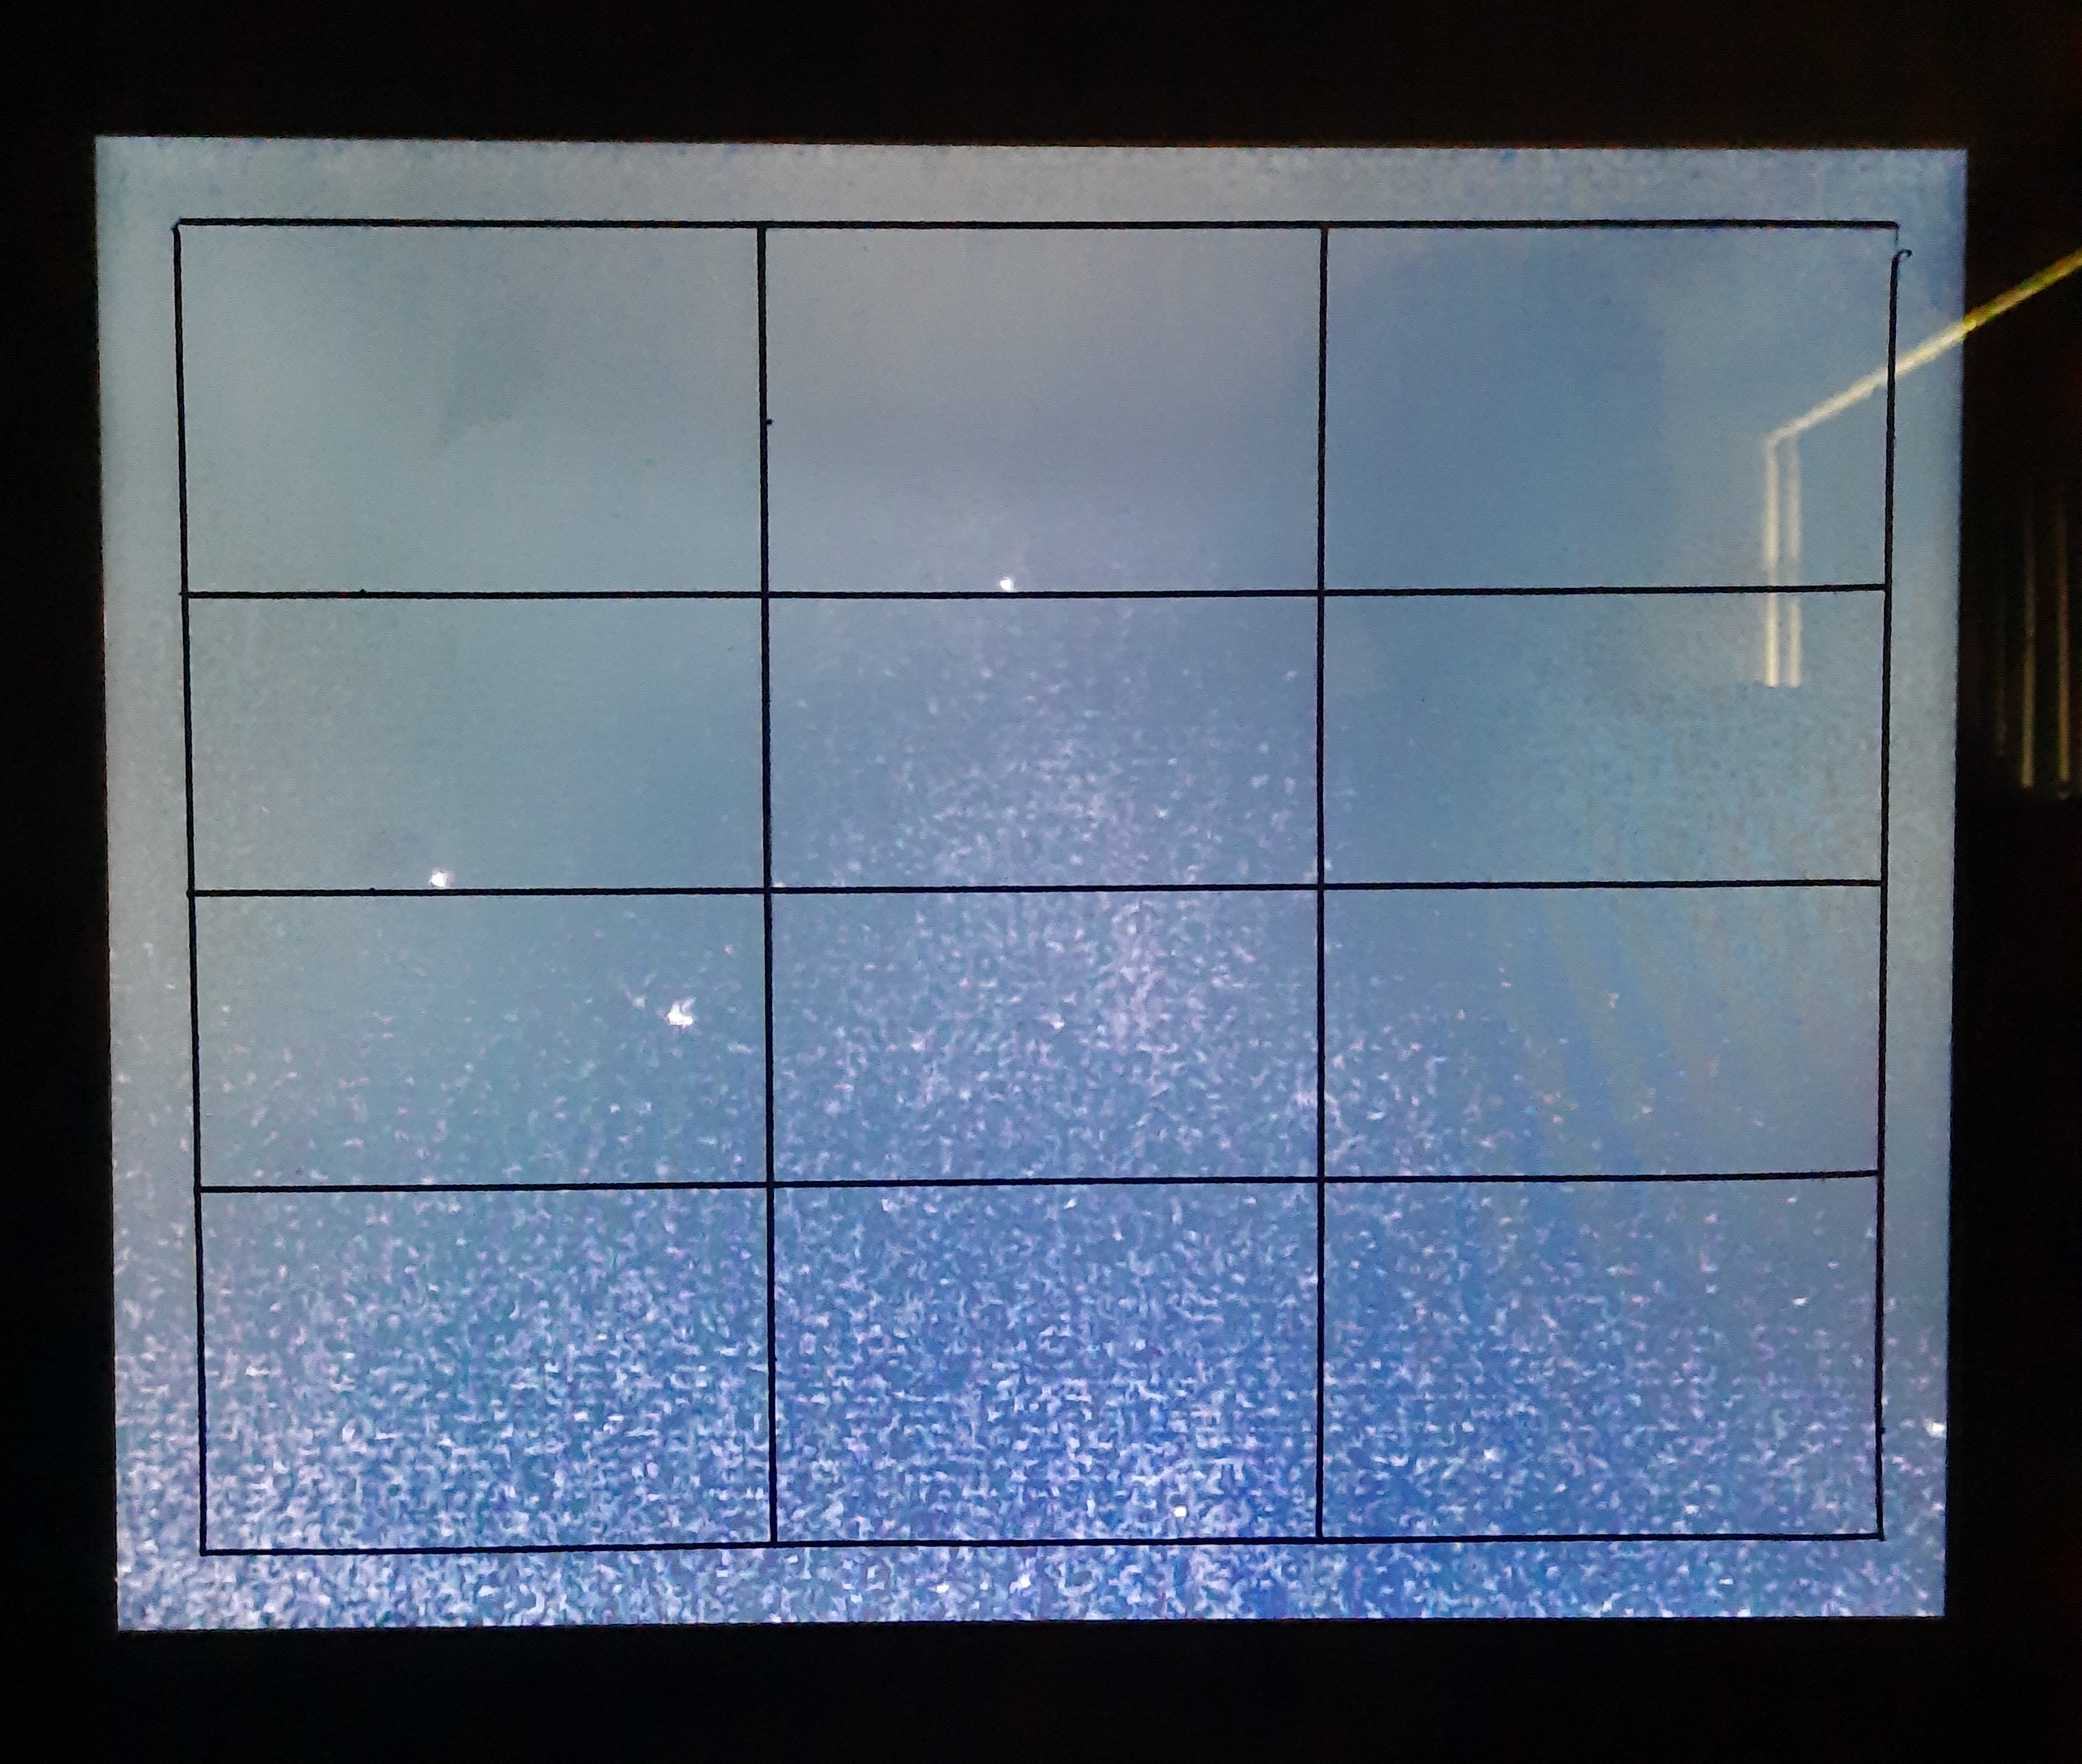
\includegraphics[width=8.5cm,height=7cm]{2} 
	\caption{Spectral line ($H_{\alpha}$) of hydrogen atom}
	\label{2}
\end{figure}

\begin{figure}[H] %  figure placement: here, top, bottom, or page
	\centering
	\includegraphics[width=9.5cm,height=7cm]{4} 
	\caption{Plot of sin $\theta$ versus wavelength to determine grating element.}
	\label{4}
\end{figure}

\begin{figure}[H] %  figure placement: here, top, bottom, or page
	\centering
	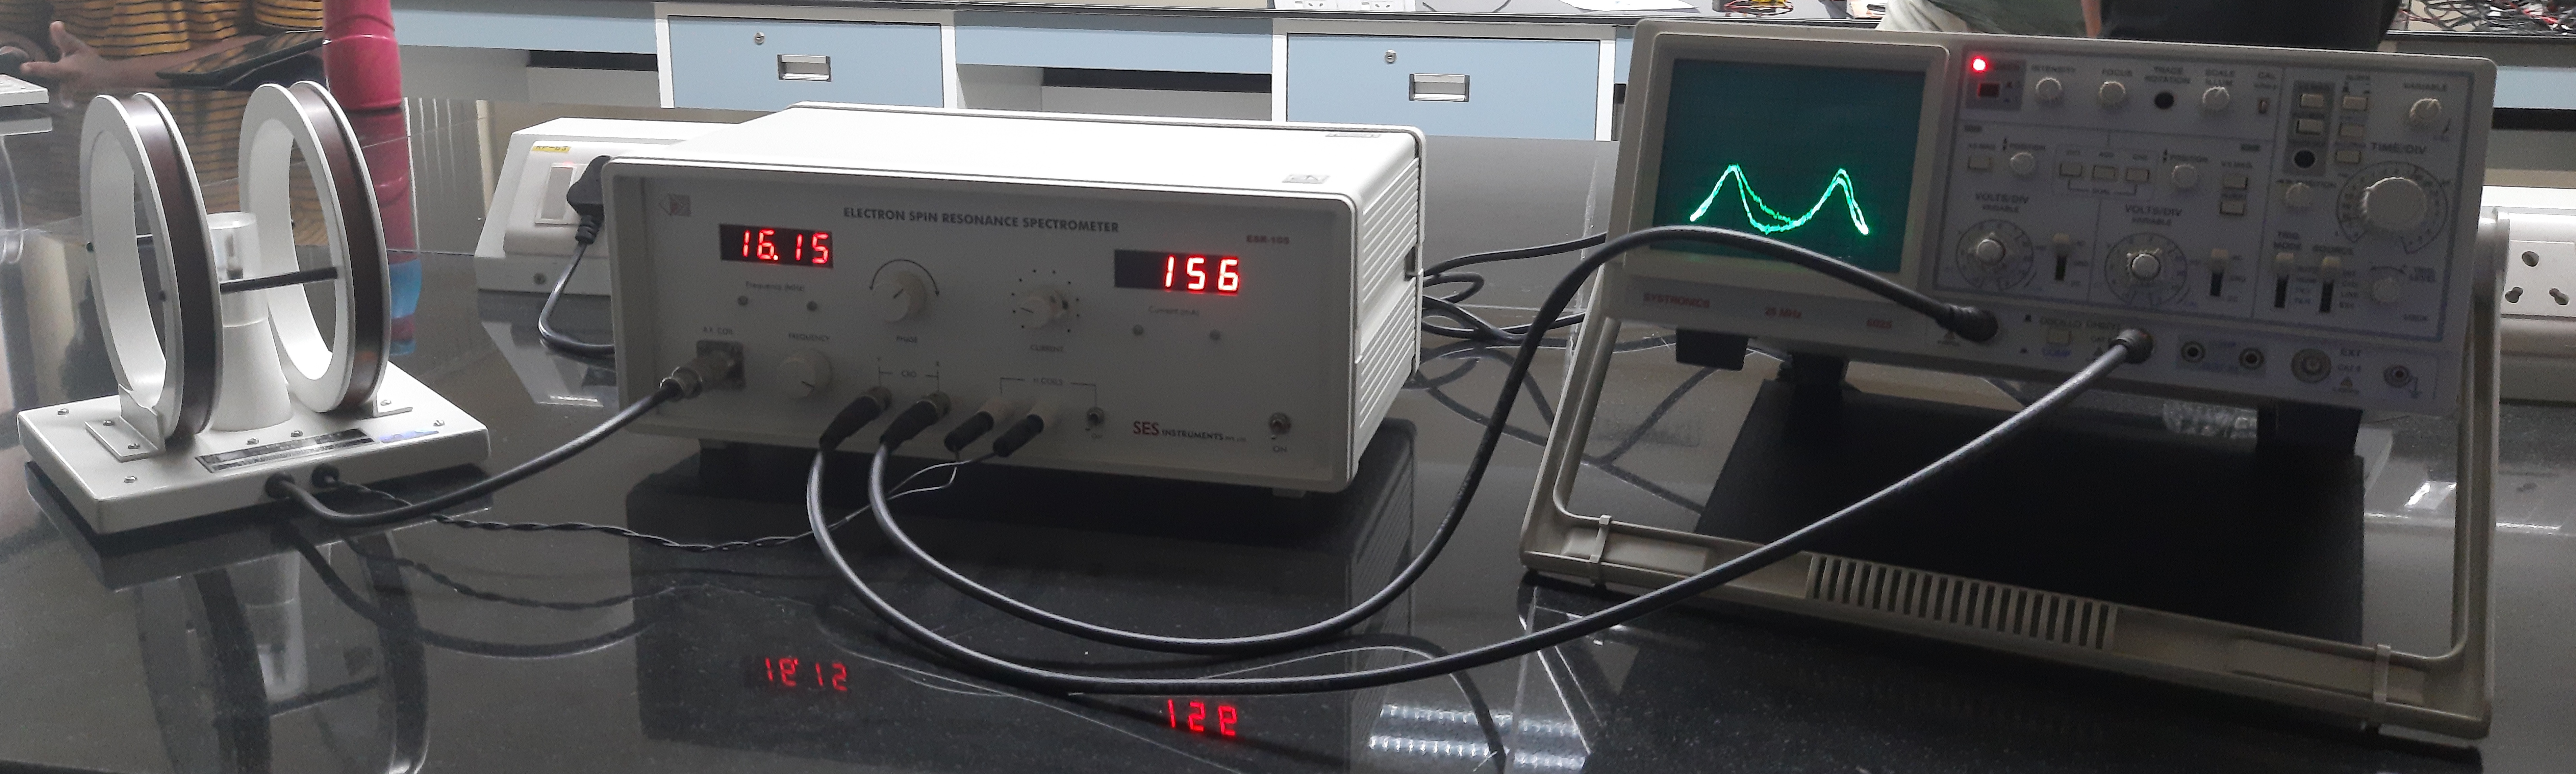
\includegraphics[width=9.5cm,height=7cm]{5} 
	\caption{Plot of difference of reciprocal of squares of energy states versus wavelength to determine Rydberg constant.}
	\label{5}
\end{figure}

From the plot of sin $\theta$ versus wavelength, we obtained grating element as $1695.24\pm18$ nm. The $\theta$ were obtained from the spectrometer. From the obtained parameter g, we calculate wavelength of spectral line from grating equation as mentioned in equation (2). We obtained the wavelength of red , greeen, violet spectral line i.e $H_\alpha$, $H_\beta$,  $H_\gamma$ as 672.17 nm, 492.81 nm, 441.90 nm, respectively. From the obtained wavelengths, we plot wavenumber (1/$\lambda$) versus difference of squares of energy states to get slope as Rydberg constant i.e $(1.0947\pm0.0180)$ $m^{-1}$

To calculate error in wavelength obtained, we have
\begin{equation}
	\frac{\delta \lambda}{ \lambda}=\sqrt{\left( \frac{\delta g}{ g}\right) ^2+\left( \frac{\delta \theta}{ \theta}\right) ^2}
\end{equation}

where $\delta g$ is error in grating element obtained from slope in Figure (5), and $\delta \theta$ is least count of spectrometer i.e 1'.

Therefore, we get $$\delta \lambda_{H_\alpha} =7.15 nm$$
$$\delta \lambda_{H_\beta} =5.25 nm$$
$$\delta \lambda_{H_\gamma} =4.71 nm$$

\section{Conclusion and Summary}
From this experiment, we determined the wavelength for spectral lines of Hydrogen atom which was found to be $H_\alpha=(672.17\pm7.15) nm$, $H_\beta=(492.81\pm5.25) nm$, $H_\beta=(441.9\pm4.71) nm$ and determined Rydberg's constant as $(1.0947\pm0.0180)\times 10^7 m^{-1}$. The literature values of three spectral lines of hydrogen in the order are 656.27 nm, 486.13 nm, 434.04 nm, respectively. The relative error of wavelengths of spectral lines is 2.42 \%, 1.37\% and 1.81\%, respectively. In case of Rydberg's constant, the relative error was found out to be 0.0182\%. This experiment was successful in determining Rydberg's constant and emission spectral lines of Hydrogen atom, since relative errors were <3\%. Still accuracy could be improved, by using instruments of lower least count,but due to certain experimental artifacts like disturbance of spectrometer while measuring angles, the ambient temperature, human errors and random errors comes into picture. The aberrations could be reduced by increasing focal length of the telescopic lens. It should be taken care that spectrometer is placed on a non slippery fixed surface.

The Balmer series is particularly useful in astronomy because they appear in numerous stellar objects due to the abundance of hydrogen in the universe, and therefore are commonly seen and relatively strong compared to lines from other elements. It is also used to determine the temperature of stars based spectral lines.

\section{References}
\begin{enumerate}
	\item {\url{https://www.niser.ac.in/sps/sites/default/files/basic_page/Balmer_series_manual.pdf}}
	\item {\url{https://en.wikipedia.org/wiki/Balmer_series}}
\end{enumerate}

\end{document}